% UAIS (Universal Access in the Information Society, Springer) submission version.
% Requires svjour3.cls (download instructions in README.md in this folder).
% Compile with: xelatex main.tex  (twice, for cross-references).

\documentclass[smallextended]{svjour3}

\smartqed  % flush right qed marks, e.g. at end of proof

\usepackage{graphicx}
\usepackage{amsmath,amssymb,amsfonts}
\usepackage{booktabs}
\usepackage{tabularx}
\usepackage{multirow}
\usepackage{float}
\usepackage{url}
\usepackage{hyperref}
\usepackage{fontspec}
\usepackage{kotex}

\journalname{Universal Access in the Information Society}

\begin{document}

\title{KOSHA-Braille: Infrastructure-Grade Accessibility for Korean Chemical Safety Information}

\titlerunning{KOSHA-Braille}

\author{Yuyong Kim}

\authorrunning{Y. Kim}

\institute{
Yuyong Kim \at
University of Wisconsin--Madison, Madison, WI 53706, USA \\
\email{ykim288@wisc.edu} \\
\textit{ORCID:} 0009-0006-4842-666X
}

\date{Received: date / Accepted: date}

\maketitle

\begin{abstract}
\textbf{Purpose.} Korean chemical safety information is produced exclusively as visual text, foreclosing visually impaired participation in chemistry-adjacent roles (research, regulation, labor advocacy, public office). This paper reports the construction, validation, and public release of a Korean Material Safety Data Sheet (MSDS) braille corpus, framed as accessibility \emph{infrastructure} under Article~9 of the UN CRPD and Article~21 of Korea's Anti-Discrimination Against Persons with Disabilities Act rather than as a usability artifact.

\textbf{Methods.} We implement a deterministic, standards-compliant Korean braille encoder for the 2017 Korean Braille Standards, apply it to the full KOSHA MSDS database accessed through the Korea Public Data Portal, and cross-validate the output against an independently developed open-source Korean braille converter. The corpus, encoder, decoder, evaluation harness, and reference web deployment are released as open source; every quantitative claim in the paper is regenerated by verification scripts shipped with the release.

\textbf{Results.} The released artifact covers 48{,}966 chemicals over a 769{,}897-row source-section database (401{,}272 sections with substantive Korean text), totaling approximately 119.3~million Korean characters and 232.3~million braille cells. The encoder agrees with the independent reference at 100\% over 442 cross-reference test cases, and the published Korean round-trip golden set is recovered at 45/45.

\textbf{Conclusion.} The contribution is an infrastructure-grade accessibility release for a previously unserved regulatory information domain. A reading-comprehension user study with visually impaired readers is identified as essential follow-up work and is deliberately scoped out of the present submission; the paper is positioned as the design, implementation, and public-release study, not as the end-user evaluation study.
\keywords{Accessibility infrastructure \and Braille \and Korean braille \and Chemical safety information \and MSDS dataset \and Disability rights}
\end{abstract}

\section{Introduction}
\label{sec:introduction}

\subsection{Accessibility as Infrastructure, Not Service}

Public accessibility systems---tactile paving, screen-door platforms, audio description on broadcast media, sign-language interpretation of parliamentary proceedings---share a structural property: their legitimacy is not contingent on per-day usage counts. They are infrastructure. Their function is to establish the conditions under which participation by persons with disabilities becomes possible at all. Evaluating such systems by market-style demand metrics conflates \emph{service} (discretionary, elastic) with \emph{infrastructure} (foundational, inelastic) and systematically undervalues low-incidence, high-stakes access.

This paper applies that lens to a domain where the gap is particularly stark: chemical safety information in the Korean regulatory regime. Material Safety Data Sheets (MSDS), internationally known as Safety Data Sheets (SDS), are mandatory documents containing hazard classifications, safe handling procedures, emergency measures, and exposure-limit information \cite{kosha_act}. They are read by chemists, industrial hygienists, emergency responders, occupational safety inspectors, injured-worker attorneys, journalists, legislators, and trade-union organizers. In South Korea these documents are produced exclusively as visual text under the Occupational Safety and Health Act \cite{kosha_act}, rendering them inaccessible to braille readers.

\subsection{The Self-Fulfilling Exclusion Problem}

The most common objection to producing domain-specific braille infrastructure is that the expected user population is small. In Korean chemical safety specifically, the observable population of visually impaired chemists, chemical engineers, or chemical-safety regulators is close to zero. We argue this observation is not evidence against infrastructure but evidence \emph{for} it: low observable participation in a profession is a predictable consequence of inaccessible professional information, not an independent fact about preference or capability.

Precedents for visually impaired participation in chemistry-adjacent work exist where infrastructure has been built or improvised: Henry ``Hoby'' Wedler, who completed a PhD in computational organic chemistry at the University of California, Davis in 2016 with the support of a 3D-printed molecular-model accessibility apparatus and subsequently founded Accessible Science to extend chemistry instruction to visually impaired students \cite{wedler}; blind legislators handling technical portfolios in multiple jurisdictions \cite{nfb_legislators}; disability-rights organizations conducting chemical-exposure litigation and regulatory advocacy. These cases demonstrate that the capability and interest are present; what is absent in the Korean case is the reading infrastructure.

The situation is further shaped by secondary readers who are not themselves chemists but must read MSDS professionally: legislative staff preparing questions for a minister of trade and industry, labor inspectors documenting an industrial accident, attorneys litigating occupational-disease claims, journalists investigating chemical-plant incidents, and civil-society organizers mobilizing around semiconductor-sector injuries. Each of these roles is a potential site of visually impaired participation, and each is foreclosed---silently---by the absence of braille MSDS infrastructure.

\subsection{Legal and Normative Basis}

Two instruments frame the obligation:

\begin{enumerate}
\item \textbf{UN Convention on the Rights of Persons with Disabilities, Article~9 (Accessibility)} \cite{crpd}: State parties shall take appropriate measures to ensure that persons with disabilities have access, on an equal basis with others, to information and communications, including information and communications technologies and systems. South Korea ratified the CRPD in 2008.

\item \textbf{Act on the Prohibition of Discrimination Against Persons with Disabilities, Article~21} \cite{kdpa}: Requires accessible-format provision of public-interest information. Chemical safety information produced by a public agency (KOSHA) under a statutory mandate falls within this scope.
\end{enumerate}

The absence of a chemical-safety braille service is therefore not a neutral market outcome; it is non-performance of an existing obligation. The question addressed by this paper is not whether such infrastructure should exist, but how to construct it at sufficient scale, fidelity, and extensibility to constitute infrastructure rather than demonstration.

\subsection{Contributions}

This paper is positioned as the \emph{design, implementation, and public-release} study for a domain-specific braille accessibility infrastructure. It is not positioned as the end-user reading-comprehension evaluation; that study is identified as essential follow-up work (Section~\ref{sec:discussion}) and the scope boundary is held explicitly throughout. Within that scope the contributions are:

\begin{enumerate}
\item \textbf{Framing contribution}: We articulate chemical safety information as an infrastructure-grade accessibility target and establish the evaluation criteria appropriate to that framing: parity of coverage, standards compliance, determinism, and extensibility, rather than adoption volume.

\item \textbf{KOSHA-Braille corpus}: A public Korean chemical safety braille corpus of 48,966 chemicals derived from a 769,897-row source-section database; the released artifact contains 401,272 sections with substantive Korean text, totaling approximately 119.3 million Korean characters and 232.3 million braille cells. To our knowledge, the largest Korean-language braille corpus of any kind released to date, and the first for any chemical-safety regime in any language.

\item \textbf{Standards-compliant deterministic encoder}: A rule-based Korean braille encoder implementing the 2017 Korean Braille Standards, cross-validated at 100\% agreement over 442 test cases against an independent open-source implementation.

\item \textbf{Mixed-script handling for technical content}: Rule-consistent braille indicator handling (Roman letter indicator, number indicator, capital indicator) for the Korean--Latin--numeric script mixture characteristic of MSDS; GHS pictogram codes resolved to descriptive Korean text for semantic rather than visual reference.

\item \textbf{Reference deployment}: A freely accessible web service providing search, real-time conversion, and file downloads in embosser-ready BRF and refreshable-display Unicode formats.

\item \textbf{Extensibility analysis} (Section~\ref{sec:extensibility}): Explicit treatment of the architectural properties that make the system a template for adjacent high-stakes accessibility domains (pharmaceutical labels, food allergens, first-aid protocols, chemical registration filings) and for adaptation across languages and regulatory regimes.
\end{enumerate}

\section{Related Work}
\label{sec:related}

\subsection{Accessibility Infrastructure}

Policy and design literature distinguish \emph{assistive services}, which respond to individual requests, from \emph{accessibility infrastructure}, which pre-installs the conditions for access. Hamraie's history of universal design \cite{hamraie} documents how accessibility provisions originated as targeted disability interventions but were progressively recognized as foundational built-environment features. Blackwell's articulation of the ``curb-cut effect'' \cite{curb_cut} generalizes the pattern: design changes initially intended for an underserved group consistently yield broader benefits, but only after the original intervention has been built ahead of demonstrated demand. Bennett and Keyes \cite{bennett_keyes} further argue that disability-related technical interventions framed in terms of marginal ``fairness'' calculations systematically miss the structural-justice dimension; the appropriate frame is whether the structural conditions for participation exist at all.

The present work positions domain-specific braille corpora for technical and regulatory information as a category of accessibility infrastructure that has been systematically underproduced, particularly outside English. Standard examples---captioning systems, public-library braille collections, audio description, sign-language interpretation of legislative proceedings---are characteristically produced in advance of measured demand and justified by rights frameworks rather than marginal-utility calculations. Within accessibility research specifically, the framings most relevant to the present work are: \emph{ability-based design} and \emph{universal usability}, which treat the absence of access as a property of the artifact rather than the user; the literature on \emph{accessible STEM} and tactile representation, which establishes the precedent that technical content (mathematics, chemistry diagrams) deserves first-class braille and tactile-graphics representation rather than only screen-reader fallbacks; and \emph{disability justice} critiques of marginal-utility framings of accessibility provision. KOSHA-Braille extends this lineage into chemical-safety regulatory documentation, a domain where neither English nor non-English first-class braille infrastructure has previously been reported.

\subsection{Braille Translation Systems and Technical-Material Braille}

Braille translation is most extensively studied for English via liblouis \cite{liblouis}, an open-source translator supporting more than 100 languages. For Korean, liblouis provides Grade~1 and Grade~2 tables based on the 2006 standards; a small number of open-source projects implement the 2017 revisions \cite{hangul_braille_converter,hanbraille}. These tools are character-level translators and do not address domain-level concerns such as consistent handling of regulatory codes, scientific notation within safety text, or large-scale corpus construction.

Beyond character-level translation, prior work on \emph{braille for technical reading} has concentrated on mathematics and STEM education---Nemeth Code and Unified English Braille for mathematical notation, with tooling such as MathML-to-braille pipelines---and on tactile-graphics support for diagrams. Comparatively little work treats large \emph{regulatory} text bodies (statutes, safety documentation, administrative rulings) as a translation target in their own right; existing accessibility provisions for such bodies are typically PDF/HTML accessibility (screen-reader friendliness) rather than first-class braille. The present work positions Korean MSDS as the regulatory analogue of mathematical braille: a domain whose readers need a deterministic, standards-compliant, large-coverage braille representation that they can consume on a refreshable display or embosser without on-the-fly translation.

\subsection{Chemical Safety Information Accessibility}

The Globally Harmonized System (GHS) \cite{ghs} standardizes visual hazard communication but specifies no braille counterpart. The European Union mandates braille on pharmaceutical packaging \cite{eu_braille}, the narrowest precedent for regulated braille in chemistry-adjacent domains; this applies to product names only, not to safety documentation. We are not aware of prior work on braille SDS/MSDS in any language.

\subsection{Korean Braille Standards}

The 2017 Korean Braille Standards \cite{ko_braille_2017} were promulgated by the Ministry of Culture, Sports and Tourism. Korean braille is syllable-structured: each Hangul block decomposes into initial consonant, vowel, and optional final consonant, with each component mapped to a fixed dot pattern. The 2017 revision expanded coverage to six domains including scientific notation and music notation.

\section{System Architecture}
\label{sec:system}

\subsection{Data Pipeline}

The system comprises four stages, illustrated in Fig.~\ref{fig:pipeline}: acquisition, extraction, encoding, and delivery.

\begin{figure}[H]
\centering

\includegraphics[width=0.95\textwidth]{fig_pipeline.pdf}
\caption{System architecture of KOSHA-Braille. MSDS data is acquired from the KOSHA public API, parsed and cleaned (including GHS pictogram conversion), encoded to Korean braille following the 2017 standards, and served through a web interface.}
\label{fig:pipeline}
\end{figure}

\begin{enumerate}
\item \textbf{Data Acquisition}: KOSHA MSDS data is retrieved via the Korea Public Data Portal REST API \cite{data_go_kr}, providing 16 standardized MSDS sections per chemical in XML format.

\item \textbf{Text Extraction}: XML responses are parsed for Korean text content. GHS pictogram references (e.g., ``GHS06.gif'') are resolved to descriptive Korean text (e.g., ``{급성독성}'') so that braille output conveys semantic hazard information rather than an unreadable filename.

\item \textbf{Braille Encoding}: Korean text is converted to Unicode braille (U+2800--U+28FF) following the 2017 Korean Braille Standards.

\item \textbf{Delivery}: A FastAPI backend serves the encoded content through a REST API; the reference single-page frontend provides search and side-by-side visual/braille viewing; downloads are offered in embosser-format BRF and Unicode \texttt{.txt}.
\end{enumerate}

\subsection{Korean Braille Encoding}

The encoding process is deterministic and lossless. Each Hangul syllable is decomposed using Unicode arithmetic into initial consonant, vowel, and final consonant, each mapping to a fixed dot pattern.

The encoder handles four character types with appropriate braille indicators:

\begin{itemize}
\item \textbf{Hangul}: direct decomposition to braille dot patterns (no indicator needed).
\item \textbf{Numbers}: number indicator (dots 3-4-5-6) followed by digit patterns.
\item \textbf{Latin letters}: Roman letter indicator (dots 3-5-6) followed by letter patterns; uppercase adds capital indicator (dot 6).
\item \textbf{Punctuation}: direct mapping to Korean braille punctuation patterns.
\end{itemize}

Double consonants use a dot-6 prefix cell followed by the base consonant pattern. Compound vowels and compound final consonants use multi-cell sequences.

Tables~\ref{tab:cho}, \ref{tab:jung}, and \ref{tab:jong} show the complete mapping for initial consonants, vowels, and final consonants, respectively. Fig.~\ref{fig:encoding_example} illustrates the full path for two representative MSDS tokens (``메탄올'' = methanol; ``인화성'' = flammable).

\begin{figure}[H]
\centering

\includegraphics[width=0.95\textwidth]{fig_encoding_example.pdf}
\caption{Worked encoding examples: each Hangul syllable is decomposed into initial/medial/final jamo (blue), then each jamo is emitted as one Korean braille cell. Empty circles denote unused dot positions in a 2$\times$3 braille cell.}
\label{fig:encoding_example}
\end{figure}

\begin{table}[H]
\centering
\caption{Initial Consonant Braille Patterns}
\label{tab:cho}
\begin{tabular}{cccc}
\toprule
Consonant & Dots & Consonant & Dots \\
\midrule
{ㄱ} & 4 & {ㅅ} & 6 \\
{ㄴ} & 1-4 & {ㅇ} & 1-2-4-5 \\
{ㄷ} & 2-4 & {ㅈ} & 4-6 \\
{ㄹ} & 5 & {ㅊ} & 5-6 \\
{ㅁ} & 1-5 & {ㅋ} & 1-2-4 \\
{ㅂ} & 4-5 & {ㅌ} & 1-2-5 \\
& & {ㅍ} & 1-4-5 \\
& & {ㅎ} & 2-4-5 \\
\bottomrule
\end{tabular}
\end{table}

\begin{table}[H]
\centering
\caption{Vowel Braille Patterns}
\label{tab:jung}
\begin{tabular}{cccc}
\toprule
Vowel & Dots & Vowel & Dots \\
\midrule
{ㅏ} & 1-2-6 & {ㅗ} & 1-3-6 \\
{ㅐ} & 1-2-3-5 & {ㅛ} & 3-4-6 \\
{ㅑ} & 3-4-5 & {ㅜ} & 1-3-4 \\
{ㅓ} & 2-3-4 & {ㅠ} & 1-4-6 \\
{ㅔ} & 1-3-4-5 & {ㅡ} & 2-4-6 \\
{ㅕ} & 1-5-6 & {ㅢ} & 2-4-5-6 \\
{ㅖ} & 3-4 & {ㅣ} & 1-3-5 \\
\bottomrule
\end{tabular}
\end{table}

\begin{table}[H]
\centering
\caption{Final Consonant Braille Patterns}
\label{tab:jong}
\begin{tabular}{cccc}
\toprule
Consonant & Dots & Consonant & Dots \\
\midrule
{ㄱ} & 1 & {ㅇ} & 2-3-5-6 \\
{ㄴ} & 2-5 & {ㅈ} & 1-3 \\
{ㄷ} & 3-5 & {ㅊ} & 2-3 \\
{ㄹ} & 2 & {ㅋ} & 2-3-5 \\
{ㅁ} & 2-6 & {ㅌ} & 2-3-6 \\
{ㅂ} & 1-2 & {ㅍ} & 2-5-6 \\
{ㅅ} & 3 & {ㅎ} & 3-5-6 \\
\bottomrule
\end{tabular}
\end{table}

\section{Dataset Description}
\label{sec:dataset}

\subsection{Source Data}

The KOSHA-Braille dataset is derived from the Korea Occupational Safety and Health Agency (KOSHA) Material Safety Data Sheet database, accessed through the Korea Public Data Portal API \cite{data_go_kr} under an authorized operational account with a daily limit of 100,000 calls per endpoint.

\subsection{Dataset Statistics}

Table~\ref{tab:stats} summarizes the dataset characteristics, recomputed directly over the released JSONL artifact. Fig.~\ref{fig:stats} shows the character distribution and the empirical text-length distribution per chemical, and Fig.~\ref{fig:section_coverage} shows per-section coverage and average length.

\begin{figure}[H]
\centering

\includegraphics[width=0.95\textwidth]{fig_dataset_stats.pdf}
\caption{Dataset characteristics, recomputed from the released JSONL ($n=48{,}966$ chemicals). (Left) character-type distribution. (Right) histogram of per-chemical total Korean text length. The bimodal shape reflects the mix of chemicals with full 16-section MSDS records and chemicals whose KOSHA records contain only a few substantive sections.}
\label{fig:stats}
\end{figure}

\begin{table}[H]
\centering
\caption{KOSHA-Braille Dataset Statistics}
\label{tab:stats}
\begin{tabular}{lr}
\toprule
Metric & Value \\
\midrule
Total chemicals & 48,966 \\
Source-DB section rows & 769,897 \\
Released non-empty sections & 401,272 \\
Avg.\ non-empty sections per chemical & 8.2 (full schema: 16) \\
Korean text (total) & 119.3 M chars \\
Korean braille (total) & 232.3 M cells \\
Mean braille:text ratio & 1.95 \\
\midrule
\multicolumn{2}{l}{\emph{Per-chemical Korean text length}} \\
\quad Mean & 2{,}436 chars \\
\quad Median & 772 chars \\
\quad Std.\ deviation & 2{,}431 chars \\
\quad Min / Max & 0 / 15{,}641 chars \\
\midrule
\multicolumn{2}{l}{\emph{Character type (of classified chars)}} \\
\quad Korean (Hangul) & 77.2\% \\
\quad Latin            & 18.3\% \\
\quad Digits           & 4.5\% \\
\bottomrule
\end{tabular}
\end{table}

\begin{figure}[H]
\centering

\includegraphics[width=0.95\textwidth]{fig_section_coverage.pdf}
\caption{Per-section coverage of the released dataset over the 16 MSDS sections defined by KOSHA. (a) number of chemicals with non-empty text for each section; sections 1 (chemical/company identification), 3 (composition), 8 (exposure controls), and 14 (transport) are populated for essentially every chemical, while regulatory and physico-chemical detail sections are populated only where the source KOSHA record carries non-placeholder content. (b) average Korean text length per section, conditional on the section being non-empty.}
\label{fig:section_coverage}
\end{figure}

\subsection{GHS Pictogram Conversion}

Original MSDS data references GHS hazard pictograms as image filenames (e.g., ``GHS06.gif''), which are meaningless in braille. The system resolves these to descriptive Korean text as shown in Table~\ref{tab:ghs}. All 147 unique H/P statement codes occurring in the database (63 H-statements, 84 P-statements) are resolved and encoded.

\begin{table}[H]
\centering
\caption{GHS Pictogram to Korean Text Conversion}
\label{tab:ghs}
\begin{tabular}{lll}
\toprule
Code & English & Korean \\
\midrule
GHS01 & Explosive & {폭발성} \\
GHS02 & Flammable & {인화성} \\
GHS03 & Oxidizing & {산화성} \\
GHS04 & Compressed gas & {고압가스} \\
GHS05 & Corrosive & {부식성} \\
GHS06 & Acute toxicity & {급성독성} \\
GHS07 & Irritant & {경고} \\
GHS08 & Health hazard & {건강유해성} \\
GHS09 & Environmental & {수생환경유해성} \\
\bottomrule
\end{tabular}
\end{table}

\subsection{Release}

The full corpus is released as a single JSONL file (943~MB) in HuggingFace-compatible schema, with a dataset card specifying provenance, license, section schema, and intended use. The encoder, decoder, and reference service are released as open-source code.

\section{Validation}
\label{sec:validation}

\subsection{Deterministic Correctness}

Korean braille encoding under the 2017 standards is a deterministic, rule-defined transformation. Each Hangul syllable decomposes unambiguously into initial, medial, and optional final, each mapping to a fixed dot pattern. Correctness therefore reduces to verifying the mapping tables and their application, rather than requiring per-output human-transcriber evaluation---an important property for infrastructure-scale corpora where sample-based human validation cannot reach global coverage.

\subsection{Cross-Reference Validation}

The encoder was validated against an independently developed open-source Korean braille converter \cite{hangul_braille_converter}. Table~\ref{tab:validation} shows the results.

\begin{table}[H]
\centering
\caption{Cross-Reference Validation Results}
\label{tab:validation}
\begin{tabular}{lrr}
\toprule
Test Set & Samples & Agreement \\
\midrule
Basic Hangul syllables & 41 & 100\% \\
Korean golden sentences & 45 & 100\% \\
MSDS chemical names & 356 & 100\% \\
\midrule
\textbf{Total} & \textbf{442} & \textbf{100\%} \\
\bottomrule
\end{tabular}
\end{table}

\subsection{Encoding Properties}

\begin{itemize}
\item \textbf{Deterministic}: identical input always produces identical output.
\item \textbf{Injective}: every distinct Hangul syllable produces a distinct Korean braille string (verified algorithmically by Hangul Unicode decomposition and confirmed across all 442 cross-reference test inputs).
\item \textbf{Standards-compliant}: all dot patterns match the 2017 Korean Braille Standards \cite{ko_braille_2017}.
\end{itemize}

\subsection{Scope of Validation}

This validation establishes correctness of the encoding mapping against a reference implementation and the published standard. Korean round-trip figures, where reported, are interpreted as decoder-path verification under explicit Korean-language dispatch and are not used as evidence against encoder correctness. With the current Korean decoder handling tightened for mixed-script, punctuation, parenthesis, quote, and numeric-span cases, the released golden set now round-trips at 45/45, the persistent stress corpus reports zero failures on 27 mixed-format cases, and repeated random sample spot-checks on the bundled sample DB currently report zero failures. This work does not include a reading-comprehension user study with visually impaired readers, which we identify as essential follow-up work. Grade~2 contracted Korean braille is not implemented; the corpus is Grade~1 throughout.

\section{Reference Deployment}
\label{sec:webservice}

\subsection{Architecture}

The web service is built on FastAPI (Python) with a single-page HTML/JavaScript frontend. SQLite stores pre-fetched MSDS XML; braille conversion is on-demand with typical response times under 500\,ms per chemical.

\subsection{API Endpoints}

\begin{itemize}
\item \texttt{GET /api/stats} -- corpus statistics
\item \texttt{GET /api/chemicals?search=} -- search by Korean name or CAS number
\item \texttt{GET /api/chemicals/\{id\}} -- full MSDS text
\item \texttt{GET /api/chemicals/\{id\}/braille} -- MSDS with Korean braille
\item \texttt{GET /api/chemicals/\{id\}/braille.txt} -- Unicode braille download
\item \texttt{GET /api/chemicals/\{id\}/braille.brf} -- BRF (embosser) download
\item \texttt{POST /api/convert} -- ad-hoc Korean$\rightarrow$braille
\end{itemize}

\subsection{User Interface and Consumption Paths}

The visual side-by-side view (Fig.~\ref{fig:webui}) is a presentation surface for sighted stakeholders (regulators, procurement officers, auditors) who must verify that braille production exists and is consistent with the Korean source. The functionally important outputs for braille readers are the downloadable BRF and Unicode files, which feed directly into: (1) refreshable braille displays over USB or Bluetooth from a local machine or phone; (2) braille embossers for hard-copy output; (3) accessible reading software on desktop and mobile. The deployment is explicitly a reference implementation, not a product; its purpose is to demonstrate that the corpus is consumable end-to-end with existing assistive hardware and software.

\begin{figure}[H]
\centering
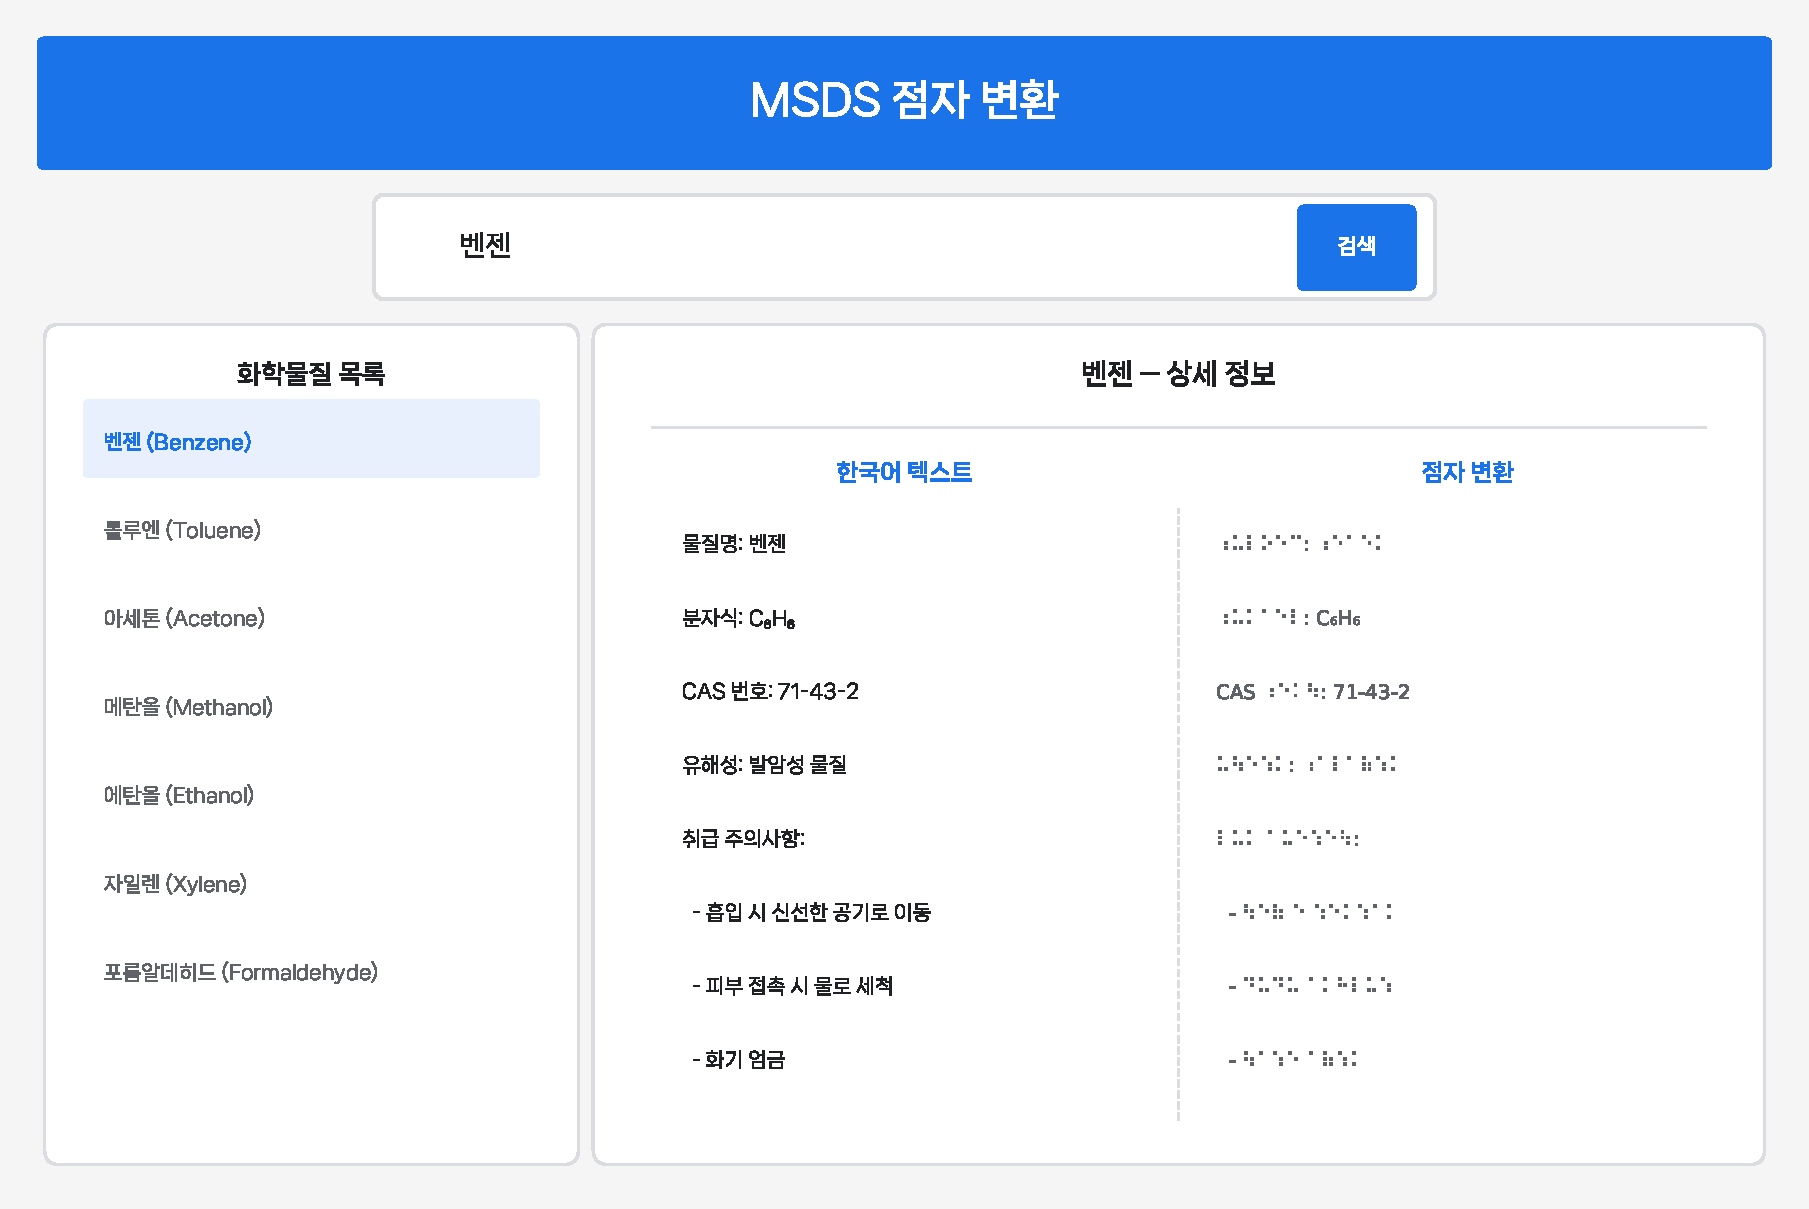
\includegraphics[width=0.95\textwidth]{fig_webui.pdf}
\caption{Web service user interface showing chemical search (top), result list (left), and side-by-side Korean text and braille display (right).}
\label{fig:webui}
\end{figure}

\section{Extensibility}
\label{sec:extensibility}

A central claim of this paper is that KOSHA-Braille is a template, not a terminus. We separate this claim into \emph{validated extensibility} (demonstrated by the current release) and \emph{prospective extensibility} (architecturally available but not yet executed at corpus scale) so that the boundary between evidence and forecast is explicit.

\subsection{Validated Extensibility (Current Release)}

The following extensions are exercised by the current release and are therefore evidence, not forecast:

\begin{itemize}
\item \textbf{Full Korean MSDS regime}: 48{,}966 chemicals, 401{,}272 non-empty sections, end-to-end through ingest, GHS resolution, braille encoding, BRF/Unicode delivery, and reference web service. This is the validated domain for the pipeline.
\item \textbf{Food allergen statements}: 19 categories enumerated in Korean food-labeling regulation, encoded and exported (\texttt{data/domain\_expansion/food\_allergens\_braille.jsonl}).
\item \textbf{First-aid and occupational-health protocols} (KISCHEM): the source DB carries 7{,}189 records; a 100-record braille export is shipped as a domain-extension demonstration (\texttt{kischem\_firstaid\_braille.jsonl}). The end-to-end path is exercised at small scale; full export is operationally tractable but is not part of the present release.
\item \textbf{CAS-keyed cross-reference}: the 13{,}445 distinct CAS numbers associated with KOSHA MSDS records, plus the 74{,}494-entry CAS$\rightarrow$PubChem~CID map bundled with the project, are encoded once and reused without re-translation, demonstrating the language-agnostic bridge into PubChem, ECHA, EPA, and OSHA registries.
\end{itemize}

\subsection{Prospective Extensibility (Architectural, Not Yet Executed)}

The following extensions are supported by the architecture but are not exercised by the current release. We mark them as forecasts so that reviewers do not read them as completed work:

\begin{itemize}
\item \textbf{Full pharmaceutical label and insert braille} (Korean Ministry of Food and Drug Safety): the narrowest international precedent (EU pharmaceutical packaging \cite{eu_braille}) is product-name only; full-label braille is a direct architectural extension but is not in the present corpus.
\item \textbf{K-REACH chemical-registration filings}: the source DB carries 47{,}344 registered substances; the pipeline would treat these as a parallel ingest path with the same encoder, but no K-REACH braille export is shipped here.
\item \textbf{Legal statutes and administrative rulings} concerning occupational safety and chemical regulation: the same template is applicable, requiring only a statute-specific ingester and the same braille encoder.
\item \textbf{Cross-regime SDS (OSHA HazCom, EU CLP/REACH, J-CHECK Japan)}: the ``structured regulatory source $\rightarrow$ language-specific braille corpus'' pattern applies; adaptation requires per-regime ingest plus substitution of the braille standard.
\end{itemize}

\subsection{Language Extensibility}

The only language-specific component is the encoder. Substitution of a rule table for another braille standard---Japanese (2001), Chinese (Mandarin Braille), English UEB, EU-country standards---preserves the remainder of the pipeline. Within the present release this is architectural (the existing encoder is Korean-specific); the substitution is mechanical but has not been executed for a second standard.

\subsection{Consumption-Format Extensibility}

The current release provides Unicode braille (U+2800--U+28FF) and BRF. Near-term extensions include Tactile SVG for embossed/thermoformed rendering, tactile-graphics derivatives of GHS pictograms, and JSON-LD annotations linking CAS and ICSC identifiers; these are listed as roadmap items, not as released components.

\subsection{Policy Extensibility}

The corpus is a concrete artifact against which policy proposals can be made: KOSHA adoption as an official accessible format; inclusion in Ministry-of-Employment-and-Labor procurement standards; integration into enterprise EHS systems with braille-embosser output.

\section{Discussion}
\label{sec:discussion}

\subsection{The Appropriate Evaluation Criterion}

We are explicit that KOSHA-Braille is not evaluated by adoption volume. The appropriate criteria for infrastructure-grade accessibility artifacts are:

\begin{enumerate}
\item Parity of coverage with the sighted-reader counterpart (here, 100\% of KOSHA MSDS records).
\item Standards compliance (verified in Section~\ref{sec:validation}).
\item Determinism and reproducibility.
\item Availability (freely accessible; no institutional or paywall gating).
\item Extensibility (Section~\ref{sec:extensibility}).
\end{enumerate}

By these criteria the present system is a substantial advance: prior state of the art for Korean chemical-safety braille was null.

\subsection{Low-Incidence High-Stakes Accessibility}

Chemical safety is one instance of a broader class of accessibility targets: technical and regulatory information domains with small observed visually impaired user populations but high consequences when access is absent. Other members of this class include legal statutes and case law, medical guidelines, standards documents, and public-administration reference materials. The economic objection to building braille infrastructure for these domains is identical in each case, and is rebutted identically: the observed user count is a function of the infrastructure, not an independent fact about it.

\subsection{Scope of Claims: What Is and Is Not Validated}
\label{sec:scope-of-claims}

We separate the validation claims into two registers so that reviewers do not have to infer the boundary.

\paragraph{Validated.}
(a) The encoder is a deterministic implementation of the 2017 Korean Braille Standards. (b) It agrees with an independently developed open-source Korean braille converter at 100\% over 442 cross-reference test cases spanning basic syllables, golden sentences, and real MSDS chemical names. (c) The released decoder path round-trips the published 45-sentence Korean golden set at 45/45 and reports zero failures on the persistent 27-case decoder stress corpus. (d) Coverage of the regulatory record is complete: every chemical present in the KOSHA MSDS database is included in the released corpus.

\paragraph{Not yet validated.}
(a) Reading comprehension by visually impaired readers. (b) Subjective usability of the BRF and Unicode outputs on refreshable displays and embossers in field conditions. (c) Sufficiency of the GHS pictogram-to-Korean text resolution for hazard recognition by braille readers (versus alternative tactile-graphics or auditory cues).

\paragraph{Why the present submission stands without (a)--(c).}
The deferred items are evaluations of \emph{the reader's interaction with the artifact}; the validated items establish \emph{that the artifact exists, is standards-conformant, has parity of coverage with the sighted-reader version, and is consumable end-to-end with standard assistive hardware}. The former category presupposes the latter. Reporting an under-powered user study at this stage would weaken rather than strengthen the contribution by misframing an infrastructure release as a usability claim. We therefore release the infrastructure now, document the boundary, and identify the user evaluation as separately powered follow-up.

\subsection{Known Limitations}

\begin{enumerate}
\item \textbf{No reading-comprehension user study} (treated separately in Section~\ref{sec:scope-of-claims}).
\item \textbf{Grade~1 only}: Korean Grade~2 contractions would shorten documents but introduce context-dependent abbreviation decisions incompatible with strict determinism at this stage.
\item \textbf{Decoder ambiguity at the choseong/jongseong boundary}: inherent to Korean braille in the abstract, but the current released Korean decode path now round-trips the published golden set at 45/45; remaining risk is therefore concentrated in unseen real-world edge cases rather than the current benchmark set.
\item \textbf{Domain terminology in translated source}: machine-translated MSDS content (where used) may carry domain-term errors that propagate to braille.
\end{enumerate}

\subsection{Maintenance and Update Model}
\label{sec:maintenance}

Because the upstream KOSHA MSDS database is itself updated, an accessibility corpus released once and never refreshed would erode toward irrelevance. We therefore commit the present release to a maintainable update model: (i) the ingest layer is parameterized by the Korea Public Data Portal API endpoint and runs idempotently against the live data source, so a re-export against a refreshed upstream is a one-command operation; (ii) the encoder, decoder, and GHS resolution layer are deterministic and self-contained Python with no closed-source dependencies, so reproduction requires only Python and the small dependency set listed in the public repository; (iii) the dataset card on HuggingFace and the GitHub repository are versioned, allowing a downstream consumer to pin to a known corpus snapshot; and (iv) the verification scripts shipped in the supplementary package regenerate every numerical claim in this paper from the released JSONL alone, so a third-party re-runner can validate any future re-export without coordination with the author. The single-maintainer risk is real and is acknowledged; the mitigations above are the structural ones available to a single-author release.

\section{Conclusion}
\label{sec:conclusion}

We have presented KOSHA-Braille as accessibility infrastructure for Korean chemical safety information: a 48{,}966-chemical, 232.3-million-cell braille corpus (401{,}272 non-empty sections released from a 769{,}897-row source-section database) produced by a deterministic, standards-compliant encoder and released publicly with a reference deployment. We argued that the appropriate framing for such work is infrastructure provision under Article~9 of the UN CRPD \cite{crpd} and Article~21 of Korea's Anti-Discrimination Against Persons with Disabilities Act \cite{kdpa}, not volume-driven service delivery. We identified and treated in Section~\ref{sec:extensibility} the architectural properties that make the system extensible across domains (pharmaceutical labels, food allergens, first-aid protocols, K-REACH filings, legal text), languages (by substitution of the braille encoder), and regulatory regimes (OSHA, CLP/REACH, J-CHECK).

The case for this kind of work should not rest on how many readers use it next month. It rests on who cannot enter a profession---whose question cannot be asked in a national assembly, whose claim cannot be pursued in court, whose investigation cannot be filed in a newsroom---when the necessary reading infrastructure does not exist. Future work includes reading-comprehension user studies with visually impaired readers, Grade~2 contracted-braille support, tactile-graphics treatment of GHS pictograms, and adoption by relevant regulators as an official accessible format.

We close by underscoring the scope boundary this paper holds throughout: the contribution is the design, validation, and public release of accessibility infrastructure; it is not a claim about end-user reading performance. Maintenance of that infrastructure beyond the present release is committed to under the model described in Section~\ref{sec:maintenance} (idempotent ingest against the live KOSHA endpoint, deterministic self-contained processing layer, versioned dataset snapshots, and third-party-reproducible verification scripts), so that the release functions as ongoing infrastructure rather than a one-off artifact.

\begin{acknowledgements}
The author thanks the Korea Occupational Safety and Health Agency (KOSHA) and the Korea Public Data Portal for maintaining open access to Material Safety Data Sheet records, and the maintainers of the independent open-source Korean braille converter \cite{hangul_braille_converter} used for the cross-reference validation reported in Section~\ref{sec:validation}.
\end{acknowledgements}

\section*{Declarations}

\paragraph{Funding}
This work received no external funding. Compute, infrastructure, and data-portal API access were self-provided.

\paragraph{Competing Interests}
The author declares no competing financial or non-financial interests.

\paragraph{Ethics and Consent}
This work involves no human subjects, no animal subjects, and no personally identifying information. Source data is publicly released regulatory material. Ethics approval, consent to participate, and consent for publication are therefore not applicable.

\paragraph{Author Contributions}
Sole author: conception, design, implementation, validation, analysis, and writing.

\paragraph{Data and Code Availability}
The dataset is released publicly on HuggingFace Datasets as \texttt{Yuyongkim/inconvenience-msds} \cite{hf_dataset}; the encoder, decoder, pipeline, web service, evaluation harness, and the verification scripts used to produce every quantitative claim in this paper are released on GitHub at \texttt{yuyongkim/inconvenience-msds} \cite{github_repo}. The MSDS source data is publicly available through the Korea Public Data Portal \cite{data_go_kr}. Dataset license: CC BY~4.0; code license: MIT.

% Springer Basic style is the journal default (numeric citations).
\bibliographystyle{spbasic}
\bibliography{refs}

\end{document}
